\documentclass[11pt, oneside]{article}   	% use "amsart" instead of "article" for AMSLaTeX format
\usepackage{geometry}                		% See geometry.pdf to learn the layout options. There are lots.
\usepackage{textcomp}
\usepackage{hyperref}  % TODO: see page 94 of latex book
\geometry{letterpaper}                   		% ... or a4paper or a5paper or ... 
%\usepackage[parfill]{parskip}    		% Activate to begin paragraphs with an empty line rather than an indent
\usepackage{graphicx}				% Use pdf, png, jpg, or eps§ with pdflatex; use eps in DVI mode
								% TeX will automatically convert eps --> pdf in pdflatex		
\usepackage{amssymb}
\usepackage{amsmath}
\usepackage{relsize}
\usepackage{parskip}


\title{CS181 / CSCI E-181 Spring 2014 Practical 4}
\author{
  David Wihl\\
  \texttt{davidwihl@gmail.com}
  \and
  Zachary Hendlin\\
  \texttt{zgh@mit.edu} 
}
%\date{}							% Activate to display a given date or no date


\begin{document}
\maketitle
\section*{Warm-Up}

The warm-up consisted of the lawn darts game using a grid of values. We used a finite horizon value iteration as the game would be certain of eventually ending if it was possible to take many throws that would hit off board yielding a zero score.

We chose to do value iteration over policy iteration because of the number of steps to execute the game were reasonable and would provide a contrast to the main problem.

The peak values occurred when it was possible to win the game with a low probability of losing (as shown in the red horizontal line in the plot). 

\begin{figure}[h!]
  \centering
  \scalebox{0.6}{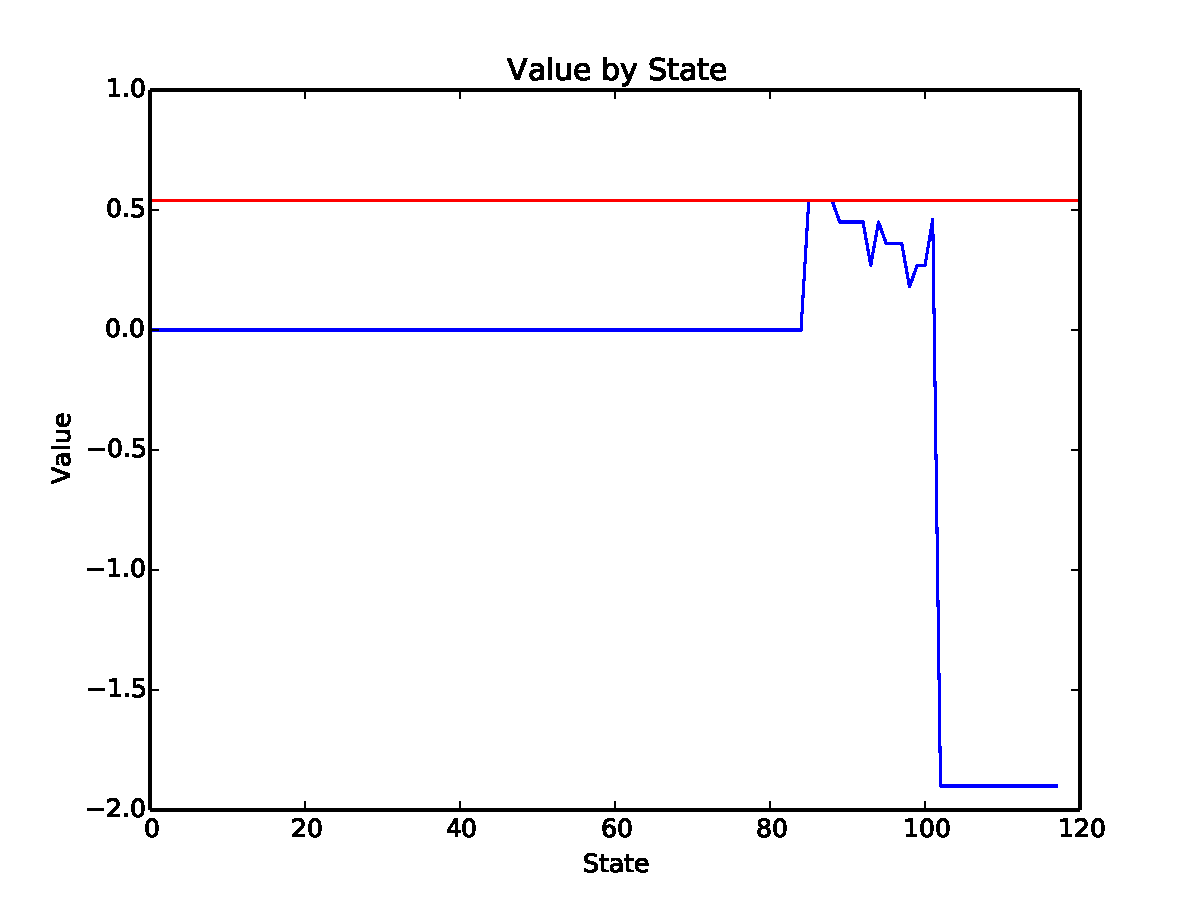
\includegraphics{values}}
 \end{figure}

\section*{Swingy Monkey}
In building a reinforcement learning system to play \textit{swingy money}, our aim was to write an \textit{action callback} function that would, for given a state as an input, provide an action (either jump or don't jump) for that period. The actions should improve as we learn more about state space and resultant rewards, making it a perfect candidate for the application of reinforcement learning.

To learn the dynamics of the system, model-free reinforcement learning was selected as the method of choice. While we considered the possiblities of trying to explicitly model the system (e.g. consider velocity, change in positions to determine angle, etc.), that approach seemed too 'engineered' in comparision to having the reinforcement learning system learn the dynamics of the system.

Our state space is given by:

\begin{itemize}

  \item Pixel of tree's bottom coordinate
  \item Pixel of tree's top coordinate
  \item Pixel distance from tree
  \item Velocity of the monkey
  \item Pixel of the bottom of the monkey
  \item Pixel of the top of the monkey \ldots

\end{itemize}

We note, however that since these pixel and velocity states are integers taking on a wide range of values:
\newline
treemin={'bot': 11, 'top': 211, 'dist': -115}
\newline
treemax={'bot': 140, 'top': 340, 'dist': 310}
\newline
monkeymin={'vel': -47, 'bot': -44, 'top': 12}
\newline
monkeymax={'vel': 18, 'bot': 364, 'top': 420}
\newline 

To deal with this 'continuous' set of values, we decided to bucket values (we explored various bucket sizes, from 2 to 100), in order to be able to visit enough of the states and learn the dynamics of the system. We found that having too many buckets would cause the system to perform poorly for many more iterations, as it takes much longer to create a non-sparse set of Q-values. So for our six variables, we have:
\begin{center}
{$2*k^{6}$} 
\end{center}
where \textit{k} is the number of bins per variable. So for k=5, we have to visit 31,250 states to visit each state,action pair. For k=10, we have visit 2,000,000 states to get one estimate of each q value.

\subsection*{Q Learning}

In Q learning, the agent aims to learn the set of rewards associated with each (state, action) pair, both for the immediate next step, as well as the discounted value of future rewards to taking a particular action.

The advantage of this approach is the flexibility it provides in being able to learn sets of optimal actions, however --as we found in this practical -- it can take many iterations to explore enough states to perform well.

We define our Q function:

\begin{equation}\label{reio}
Q(s,a) = R(s,a) +  \gamma (\sum_{s \prime} P(s\prime | s, a) \max_{a\prime \epsilon A} Q(s \prime, a \prime)
\end{equation}

The update of the Q fuction at each time set for a (state, action) pair is:

\begin{equation}\label{reio}
Q(s,a)_new = Q(s,a) +  \alpha (r + \gamma \max_{a\prime \epsilon A} Q(s \prime, a \prime) - Q(s,a))
\end{equation}
\newline
where:
\newline
$\gamma$ = discount factor, between 0 and 1 (inclusive)
\newline
$\alpha$ = learning rate, between 0 and 1 (inclusive)
\newline

\subsection*{Approach}

For our first time step, we don't know anything about the Q function value and so take a random action.

For all subsequent time steps, we compute the Q value as given above for the previous state's action and reward. We then determine, for the state the agent is, which action (jump or no jump) has a higher Q-value in the dictionary of Q-values that we have updated at each step.

Since the Q-values are not populated for state-action pairs we have not visited, we set all unvisited state-action Q-value pairs to zero at initialization.

In order to caputure the fact that there is some stochastic element to the outcome (as we know that the game engine, for instance, randomizes state-reward mappings), we choose the opposite of the optimal action a very small fraction or the time (.01 percent of the time).

\section*{Results}
With only minor parameter tuning, $\alpha = 0.05$,$\gamma = 0.9$, 5 bins, P(try random)=.001, and training on 2000 game epochs, we were able to achieve a maximum score of 193 and an average score of 16.986.

For runs 2000 to 4000, we were able to achieve a max score of 210, and an average score of 18.36

Runs 2000 to 4000 are shown below on the x-axis, with score on the y-axis.

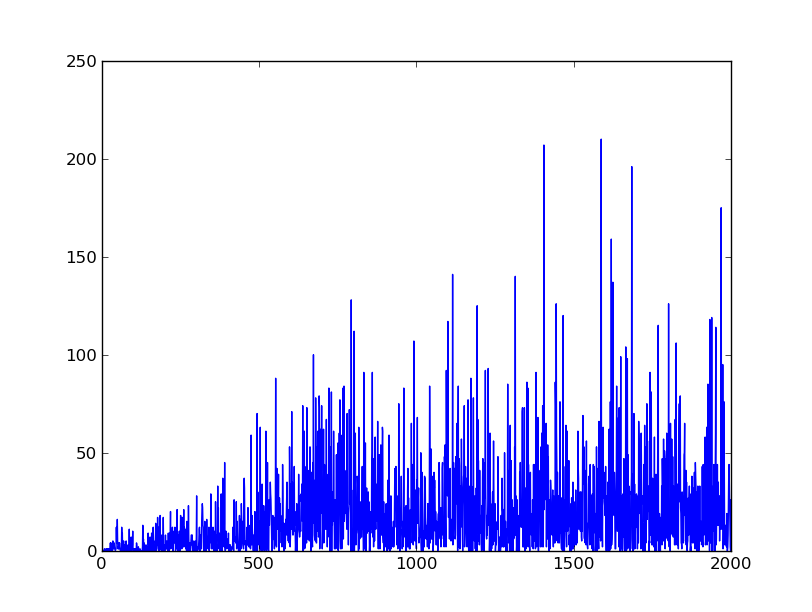
\includegraphics[scale=.5]{graph2}
\newline
As expected, in the intial epochs, the RL-based gameplay doesn't do very well as all state action pairs have a Q-value of zero. With more iterations, we see that the scores improve substantially.

Having a sufficiently large number of visits to each state and action is key to the Q-learning approach performing well.

\begin{thebibliography}{1}

 \bibitem{item1}bibitem1 
 
  \end{thebibliography}

\end{document}  
